\documentclass[12pt,a4paper]{article}
\usepackage[utf8]{inputenc} % inutile avec XeLaTeX/LuaLaTeX
\usepackage[T1]{fontenc}
\usepackage{amsmath,amssymb,mathrsfs,tikz,times,pifont}
\usepackage{enumitem}
\usepackage{multicol}
\usepackage{lmodern}
\newcommand\circitem[1]{%
\tikz[baseline=(char.base)]{
\node[circle,draw=gray, fill=red!55,
minimum size=1.2em,inner sep=0] (char) {#1};}}
\newcommand\boxitem[1]{%
\tikz[baseline=(char.base)]{
\node[fill=cyan,
minimum size=1.2em,inner sep=0] (char) {#1};}}
\setlist[enumerate,1]{label=\protect\circitem{\arabic*}}
\setlist[enumerate,2]{label=\protect\boxitem{\alph*}}
\everymath{\displaystyle}
\usepackage[left=1cm,right=1cm,top=1cm,bottom=1.7cm]{geometry}
\usepackage[colorlinks=true, linkcolor=blue, urlcolor=blue, citecolor=blue]{hyperref}
\usepackage{array,multirow}
\usepackage[most]{tcolorbox}
\usepackage{varwidth}
\usepackage{float}
\tcbuselibrary{skins,hooks}
\usetikzlibrary{patterns}

\newtcolorbox{exa}[2][]{enhanced,breakable,before skip=2mm,after skip=5mm,
colback=yellow!20!white,colframe=black!20!blue,boxrule=0.5mm,
attach boxed title to top left ={xshift=0.6cm,yshift*=1mm-\tcboxedtitleheight},
fonttitle=\bfseries,
title={#2},#1,
boxed title style={frame code={
\path[fill=tcbcolback!30!black]
([yshift=-1mm,xshift=-1mm]frame.north west)
arc[start angle=0,end angle=180,radius=1mm]
([yshift=-1mm,xshift=1mm]frame.north east)
arc[start angle=180,end angle=0,radius=1mm];
\path[left color=tcbcolback!60!black,right color = tcbcolback!60!black,
middle color = tcbcolback!80!black]
([xshift=-2mm]frame.north west) -- ([xshift=2mm]frame.north east)
[rounded corners=1mm]-- ([xshift=1mm,yshift=-1mm]frame.north east)
-- (frame.south east) -- (frame.south west)
-- ([xshift=-1mm,yshift=-1mm]frame.north west)
[sharp corners]-- cycle;
},interior engine=empty,
},interior style={top color=yellow!5}}

\usepackage{fancyhdr}
\usepackage{eso-pic}
\usepackage{tkz-tab}
\AddToShipoutPicture{
    \AtTextCenter{%
        \makebox[0pt]{\rotatebox{80}{\textcolor[gray]{0.7}{\fontsize{5cm}{5cm}\selectfont PGB}}}
    }
}

\usepackage{verbatim}
\usepackage{istgame}
\usepackage{color,soul}

\usepackage{amsmath}
\usepackage{amsfonts}
\usepackage{amssymb}
\usepackage{systeme}
\usepackage{tkz-tab}
\usepackage{tikz}
\usetikzlibrary{arrows}
\newcounter{exemple} % Compteur pour les questions

% Définir la commande pour afficher une question numérotée
\newcommand{\exemple}{%
  \refstepcounter{exemple}%
  \textbf{\textcolor{green}{Exemple \theexemple :}} \ignorespaces
}
%---------------------------------------
\definecolor{myorange}{rgb}{1.0, 0.8, 0.0}

% Définir un compteur pour les exercices d'application
\newcounter{exerciceapp}

% Définir la commande pour afficher un exercice d'application numéroté
\newcommand{\exerciceapp}{%
  \refstepcounter{exerciceapp}%
  \textbf{\textcolor{myorange}{Exercice d'application \theexerciceapp :}} \ignorespaces
}
%--------------------------------------
% Définir un compteur pour les exercices d'application
\newcounter{correction}

% Définir la commande pour afficher un correction exercice d'application numéroté
\newcommand{\correction}{%
  \refstepcounter{correction}%
  \textbf{\textcolor{myorange}{Correction \thecorrection :}} \ignorespaces
}
%--------------------------------------
% Commande pour ajouter du texte en arrière-plan
\usepackage{fancyhdr}
\usepackage{eso-pic}
\usepackage{diagbox}
\usepackage{xcolor} % Pour ajouter les couleurs

% Définition d'un rouge foncé similaire à l'encre du cahier
\definecolor{darkred}{rgb}{0.7, 0, 0}
\definecolor{darkgreen}{rgb}{0, 0.7, 0}
%\usepackage{tkz-tab}
\AddToShipoutPicture{
    \AtTextCenter{%
        \makebox[0pt]{\rotatebox{80}{\textcolor[gray]{0.7}{\fontsize{5cm}{5cm}\selectfont PGB}}}
    }
}
%This command takes a colour as an optional argument; the default colour is black.
\usetikzlibrary{shapes.geometric,fit}
\newcommand{\myul}[2][black]{\setulcolor{#1}\ul{#2}\setulcolor{black}}
\newcommand\tab[1][1cm]{\hspace*{#1}}

\begin{document}
% En-tête personnalisée
\begin{center}
    \Large\textbf{\underline{\textcolor{red}{Fonctions-Applications}}}\\[-0.1cm]
    \normalsize\textbf{Prof : M. BA} \hfill \textbf{Classe : 1er S2}\\[-0.1cm]
    \textbf{Année scolaire : 2026 -- 2027}
\end{center}

\section*{\color{red}Chapitre II : Fonctions - Applications}

\subsection*{\color{darkred}I. Notion de fonctions}

\subsubsection*{\color{darkgreen} 1) Définitions et exemples}

\paragraph{\color{darkred}a) Définition :}~\\
On appelle \color{darkred}fonction\color{black}, toute relation \color{darkred}$f$\color{black} entre 2 ensembles {\color{darkred}$A$} et {\color{darkred}$B$} telle que à tout élément {\color{darkred}$x$} de {\color{darkred}$A$} on associe au plus un élément {\color{darkred}$y$} de {\color{darkred}$B$}. Cela veut dire 1 image ou pas d'image uniquement.

Si {\color{darkred}$x$} est associé à {\color{darkred}$y$} ($x \in A$ et $y \in B$), on note alors :
\[
\boxed{f(x) = y}
\]

\begin{itemize}
    \item {\color{darkred}$y$} est appelé image de {\color{darkred}$x$} par la fonction {\color{darkred}$f$},
    \item et {\color{darkred}$x$} est un antécédent de {\color{darkred}$y$} par {\color{darkred}$f$}.
    \item {\color{darkred}$A$} est l'ensemble de départ de la fonction {\color{darkred}$f$} et {\color{darkred}$B$} son ensemble d'arrivée.
\end{itemize}

\paragraph{\color{darkred}b) Exemples:}~\\

\begin{center}
\begin{minipage}{0.45\textwidth}
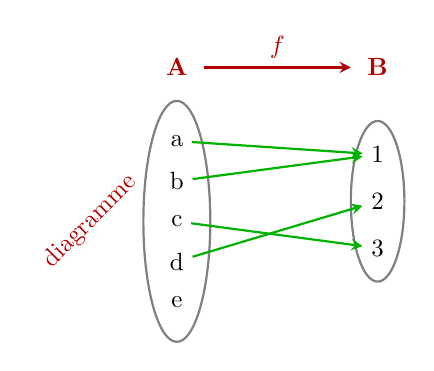
\begin{tikzpicture}[scale=0.85, every node/.style={scale=0.9}]
    % Label "diagramme" incliné en rouge à gauche
    \node[text=darkred, rotate=45] at (-1.3,0) {diagramme};

    % Ensembles A et B
    \node[text=darkred, font=\bfseries] at (0,2.3) {A};
    \node[text=darkred, font=\bfseries] at (3,2.3) {B};
    
    % Flèche f de A vers B
    \draw[->, >=stealth, color=darkred, thick] (0.4,2.3) -- node[above] {$f$} (2.6,2.3);

    % Enveloppes (patates) pour A et B
    \draw[thick, color=gray] (0,0) ellipse (0.5cm and 1.8cm);
    \draw[thick, color=gray] (3,0.3) ellipse (0.4cm and 1.2cm);

    % Éléments de l'ensemble A
    \node (a) at (0,1.2) {a};
    \node (b) at (0,0.6) {b};
    \node (c) at (0,0) {c};
    \node (d) at (0,-0.6) {d};
    \node (e) at (0,-1.2) {e};

    % Éléments de l'ensemble B
    \node (1) at (3,1.0) {1};
    \node (2) at (3,0.3) {2};
    \node (3) at (3,-0.4) {3};

    % Flèches de correspondance (en vert comme sur l'image)
    \draw[->, >=stealth, color=darkgreen, thick] (a) -- (1);
    \draw[->, >=stealth, color=darkgreen, thick] (b) -- (1);
    \draw[->, >=stealth, color=darkgreen, thick] (c) -- (3);
    \draw[->, >=stealth, color=darkgreen, thick] (d) -- (2);

\end{tikzpicture}
\end{minipage}
\begin{minipage}{0.45\textwidth}
    $\begin{aligned}
    f(a) &= 1 \\
    f(b) &= 1 \\
    f(c) &= 3 \\
    f(d) &= 2
    \end{aligned}$
    
    \vspace{0.3cm}
    $e$ n'a pas d'image par $f$.
\end{minipage}
\end{center}

\vspace{0.5cm}
A tout élément de {\color{darkred}$A$} on associe au plus un élément de {\color{darkred}$B$}. Donc, la relation {\color{darkred}$f$} ainsi définie est une {\color{darkred}fonction}.

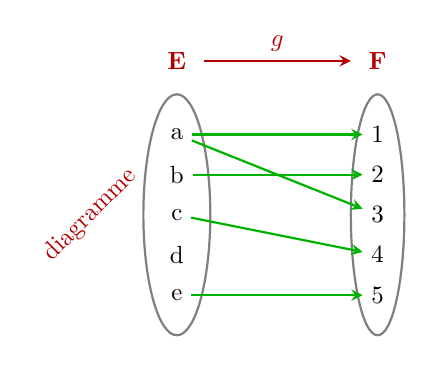
\begin{tikzpicture}[scale=0.85, every node/.style={scale=0.9}]
    % Label "diagramme" incliné en rouge à gauche
    \node[text=darkred, rotate=45] at (-1.3,0) {diagramme};

    % Ensembles E et F
    \node[text=darkred, font=\bfseries] at (0,2.3) {E};
    \node[text=darkred, font=\bfseries] at (3,2.3) {F};
    
    % Flèche g de E vers F
    \draw[->, >=stealth, color=darkred, thick] (0.4,2.3) -- node[above] {$g$} (2.6,2.3);

    % Enveloppes (patates) pour E et F
    \draw[thick, color=gray] (0,0) ellipse (0.5cm and 1.8cm);
    \draw[thick, color=gray] (3,0) ellipse (0.4cm and 1.8cm);

    % Éléments de l'ensemble E
    \node (a) at (0,1.2) {a};
    \node (b) at (0,0.6) {b};
    \node (c) at (0,0) {c};
    \node (d) at (0,-0.6) {d};
    \node (e) at (0,-1.2) {e};

    % Éléments de l'ensemble F
    \node (1) at (3,1.2) {1};
    \node (2) at (3,0.6) {2};
    \node (3) at (3,0) {3};
    \node (4) at (3,-0.6) {4};
    \node (5) at (3,-1.2) {5};

    % Flèches de correspondance en vert
    \draw[->, >=stealth, color=darkgreen, thick] (a) -- (1);
    \draw[->, >=stealth, color=darkgreen, thick] (a) -- (3);
    \draw[->, >=stealth, color=darkgreen, thick] (b) -- (2);
    \draw[->, >=stealth, color=darkgreen, thick] (c) -- (4);
    \draw[->, >=stealth, color=darkgreen, thick] (e) -- (5);

\end{tikzpicture}

\vspace{0.3cm}
{\color{darkred}$g$} n'est pas une fonction car on a associé à {\color{darkred}$a \in E$}, {\color{darkred}2 éléments} $1$ et $3$ de $F$.

\paragraph{\color{darkred} Remarque: \hrulefill}~\\

\begin{itemize}
    \item[$\bullet$] Si {\color{darkred}$B \subset \mathbb{R}$} alors {\color{darkred}$f$} est appelée une {\color{darkred}fonction numérique}.
    \item[$\bullet$] Si {\color{darkred}$A \subset \mathbb{R}$} alors {\color{darkred}$f$} est appelée une {\color{darkred}fonction à variable réelle}.
    \item[$\bullet$] Si {\color{darkred}$A \subset \mathbb{R}$ et $B \subset \mathbb{R}$} alors {\color{darkred}$f$} est appelée une {\color{darkred}fonction numérique à variable réelle}.
\end{itemize}

\subsubsection*{\color{darkgreen} 2) Ensemble de définition}

Soit {\color{darkred}$f$} une fonction \quad $\begin{aligned} f : A &\rightarrow B \\ x &\mapsto y = f(x) \end{aligned}$

L'{\color{darkred}ensemble de définition} de {\color{darkred}$f$} noté {\color{darkred}$\mathcal{D}_f$} est l'ensemble des éléments de {\color{darkred}$A$} qui ont une image par {\color{darkred}$f$} dans {\color{darkred}$B$}.

\paragraph{Exemple : \hrulefill}~\\
\begin{itemize}
    \item[$\bullet$] Dans le $1^{\text{er}}$ diagramme, l'ensemble de définition de $f$ est : $\boxed{\mathcal{D}_f = \{a ; b ; c ; d\}}$
    
    \item[$\bullet$] $\begin{aligned} f : \mathbb{R} &\rightarrow \mathbb{R} \\ x &\mapsto 2x^3 - 5x + 3 \end{aligned}$ \\
    {\color{darkred}$\mathcal{D}_f = \mathbb{R}$}
    
    \item[$\bullet$] $\begin{aligned} f : \mathbb{R} &\rightarrow \mathbb{R} \\ x &\mapsto \frac{2x+5}{x^2-4} \end{aligned} \implies f \text{ existe ssi } x^2-4 \neq 0, \text{ posons } x^2-4 = 0$ \\
    \phantom{$\begin{aligned} f : \mathbb{R} &\rightarrow \mathbb{R} \\ x &\mapsto \frac{2x+5}{x^2-4} \end{aligned} \implies f \text{ existe ssi } x^2-4 \neq 0, \text{ posons }$} $x = \pm 2$ \\
    {\color{darkred}$\mathcal{D}_f = \mathbb{R} \setminus \{-2 ; 2\} = ]-\infty ; -2[ \cup ]-2 ; 2[ \cup ]2 ; +\infty[$}
    
    \item[$\bullet$] $\begin{aligned} f : \mathbb{R} &\rightarrow \mathbb{R} \\ x &\mapsto \sqrt{x-1} \end{aligned}$ \\
    $f \text{ existe ssi } x-1 \geq 0 \implies x \geq 1$ \\
    {\color{darkred}$\mathcal{D}_f = [1 ; +\infty[$}
\end{itemize}

\subsubsection*{\color{darkgreen} 3) Restriction - prolongement d'une fonction}
\paragraph{\color{darkred}a) Définition :}~\\

Soit $f$ une fonction définie de $A$ vers $B$.

Étant donné que {\color{darkred}$D \subset A$}, la {\color{darkred}restriction} de $f$ à $D$ notée {\color{darkred}$f/_D$} est la fonction :
$$
\begin{aligned}
f/_D : D &\rightarrow B \\
x &\mapsto y = f(x)
\end{aligned}
$$
{\color{darkred}$f$} est alors appelée le {\color{darkred}prolongement} de $f/_D$ à $A$.

\paragraph{Exemple :}~\\
Soit $f$ la fonction représentée par le diagramme ci-dessous :

\begin{center}
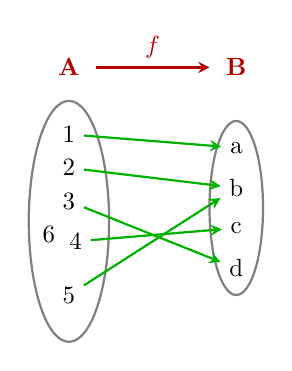
\begin{tikzpicture}[scale=0.85, every node/.style={scale=0.9}]
    % --- DIAGRAMME 1 : f ---
    % Ensembles A et B
    \node[text=darkred, font=\bfseries] at (0,2.3) {A};
    \node[text=darkred, font=\bfseries] at (2.5,2.3) {B};
    \draw[->, >=stealth, color=darkred, thick] (0.4,2.3) -- node[above] {$f$} (2.1,2.3);

    % Patates A et B
    \draw[thick, color=gray] (0,0) ellipse (0.6cm and 1.8cm);
    \draw[thick, color=gray] (2.5,0.2) ellipse (0.4cm and 1.3cm);

    % Éléments
    \node (a1) at (0,1.3) {1};
    \node (a2) at (0,0.8) {2};
    \node (a3) at (0,0.3) {3};
    \node (a6) at (-0.3,-0.2) {6};
    \node (a4) at (0.1,-0.3) {4};
    \node (a5) at (0,-1.1) {5};

    \node (ba) at (2.5,1.1) {a};
    \node (bb) at (2.5,0.5) {b};
    \node (bc) at (2.5,-0.1) {c};
    \node (bd) at (2.5,-0.7) {d};

    % Flèches
    \draw[->, >=stealth, color=darkgreen, thick] (a1) -- (ba);
    \draw[->, >=stealth, color=darkgreen, thick] (a2) -- (bb);
    \draw[->, >=stealth, color=darkgreen, thick] (a3) -- (bd);
    \draw[->, >=stealth, color=darkgreen, thick] (a4) -- (bc);
    \draw[->, >=stealth, color=darkgreen, thick] (a5) -- (bb);
\end{tikzpicture}

\vspace{0.5cm}

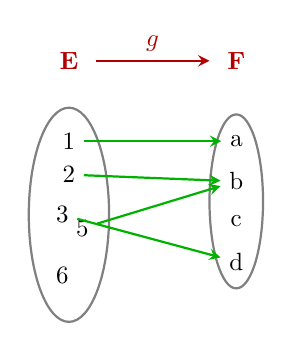
\begin{tikzpicture}[scale=0.85, every node/.style={scale=0.9}]
    % --- DIAGRAMME 2 : g ---
    % Ensembles E et F
    \node[text=darkred, font=\bfseries] at (0,2.3) {E};
    \node[text=darkred, font=\bfseries] at (2.5,2.3) {F};
    \draw[->, >=stealth, color=darkred, thick] (0.4,2.3) -- node[above] {$g$} (2.1,2.3);

    % Patates E et F
    \draw[thick, color=gray] (0,0) ellipse (0.6cm and 1.6cm);
    \draw[thick, color=gray] (2.5,0.2) ellipse (0.4cm and 1.3cm);

    % Éléments
    \node (e1) at (0,1.1) {1};
    \node (e2) at (0,0.6) {2};
    \node (e3) at (-0.1,0.0) {3};
    \node (e5) at (0.2,-0.2) {5};
    \node (e6) at (-0.1,-0.9) {6};

    \node (fa) at (2.5,1.1) {a};
    \node (fb) at (2.5,0.5) {b};
    \node (fc) at (2.5,-0.1) {c};
    \node (fd) at (2.5,-0.7) {d};

    % Flèches
    \draw[->, >=stealth, color=darkgreen, thick] (e1) -- (fa);
    \draw[->, >=stealth, color=darkgreen, thick] (e2) -- (fb);
    \draw[->, >=stealth, color=darkgreen, thick] (e3) -- (fd);
    \draw[->, >=stealth, color=darkgreen, thick] (e5) -- (fb);
\end{tikzpicture}
\end{center}

Soit $E = \{1 ; 2 ; 3 ; 5 ; 6\}$, il est clair que {\color{darkred}$E \subset A$} donc {\color{darkred}$g$ est une restriction} de $f$ sur $E$ ou {\color{darkred}$f$ est un prolongement} de $g$ à $A$.

On donne $f(x) = |x - 1|$. Écrire $f$ sans le symbole de la valeur absolue puis donner la restriction de $f$ sur $]1 ; +\infty[$.

$$
f(x) = \begin{cases} 
-x + 1 \text{ si } x < 1 \\ 
x - 1 \text{ si } x > 1 \\ 
0 \text{ si } x = 1 
\end{cases} 
\implies \boxed{\left. f(x) \right|_{]1 ; +\infty[} = x - 1}
$$

\section*{\underline{\textbf{\textcolor{darkred}{I. Notion d'application}}}}
\subsection*{\underline{\textbf{\textcolor{darkgreen}{1. Définition et exemples}}}}

\paragraph{\color{darkred}a) Définition :}~\\


On appelle \textcolor{darkred}{\textbf{application}} d'un ensemble $A$ vers un ensemble $B$
toute relation de $A$ vers $B$ telle que \textcolor{darkgreen}{\textbf{à tout élément de $A$,
on associe un et un seul élément de $B$}}.

Autrement dit, chaque élément de $A$ possède une unique image dans $B$.


\paragraph{\color{darkred}b) Exemple :}~\\

La relation qui à chaque élève de la $1^{\text{ère}}$ S$_2$ du lycée
associe son âge est une \textcolor{darkred}{\textbf{application}}.

En effet, un élève ne peut avoir qu'un seul et unique âge.

\begin{center}

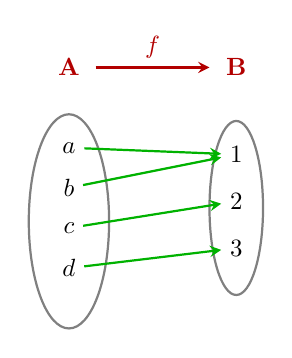
\begin{tikzpicture}[scale=0.85, every node/.style={scale=0.9}]

    % --- DIAGRAMME : f ---

    % Ensembles A et B
    \node[text=darkred, font=\bfseries] at (0,2.3) {A};
    \node[text=darkred, font=\bfseries] at (2.5,2.3) {B};

    % Flèche indiquant l'application
    \draw[->, >=stealth, color=darkred, thick]
        (0.4,2.3) -- node[above] {$f$} (2.1,2.3);

    % Patates A et B
    \draw[thick, color=gray]
        (0,0) ellipse (0.6cm and 1.6cm);

    \draw[thick, color=gray]
        (2.5,0.2) ellipse (0.4cm and 1.3cm);

    % Éléments de A
    \node (a) at (0,1.1) {$a$};
    \node (b) at (0,0.5) {$b$};
    \node (c) at (0,-0.1) {$c$};
    \node (d) at (0,-0.7) {$d$};

    % Éléments de B
    \node (e1) at (2.5,1.0) {$1$};
    \node (e2) at (2.5,0.3) {$2$};
    \node (e3) at (2.5,-0.4) {$3$};

    % Flèches
    \draw[->, >=stealth, color=darkgreen, thick]
        (a) -- (e1);

    \draw[->, >=stealth, color=darkgreen, thick]
        (b) -- (e1);

    \draw[->, >=stealth, color=darkgreen, thick]
        (c) -- (e2);

    \draw[->, >=stealth, color=darkgreen, thick]
        (d) -- (e3);

\end{tikzpicture}

\end{center}

On a :

\[
\begin{aligned}
f(a) &= 1,\\
f(b) &= 1,\\
f(c) &= 2,\\
f(d) &= 3.
\end{aligned}
\]

Cependant, un élément de $B$ peut avoir plusieurs antécédents dans $A$,
ou même n'avoir aucun antécédent.

\paragraph{\color{darkred}c) Contre-exemple : :}~\\

$f$ est une application car tout élément de départ est inclus dans son
ensemble de définition.

À chaque élément de $A$ on associe un et un seul élément de $B$.

\begin{center}

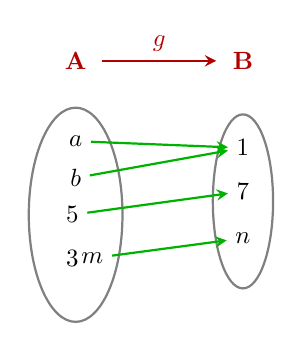
\begin{tikzpicture}[scale=0.85, every node/.style={scale=0.9}]

    % --- DIAGRAMME : g ---

    % Ensembles A et B
    \node[text=darkred, font=\bfseries] at (0,2.3) {A};
    \node[text=darkred, font=\bfseries] at (2.5,2.3) {B};

    % Flèche indiquant la relation
    \draw[->, >=stealth, color=darkred, thick]
        (0.4,2.3) -- node[above] {$g$} (2.1,2.3);

    % Patates A et B
    \draw[thick, color=gray]
        (0,0) ellipse (0.7cm and 1.6cm);

    \draw[thick, color=gray]
        (2.5,0.2) ellipse (0.45cm and 1.3cm);

    % Éléments de A
    \node (a) at (0,1.1) {$a$};
    \node (b) at (0,0.55) {$b$};
    \node (c) at (-0.05,0.0) {$5$};
    \node (d) at (-0.05,-0.65) {$3$};
    \node (m) at (0.25,-0.65) {$m$};

    % Éléments de B
    \node (e1) at (2.5,1.0) {$1$};
    \node (e2) at (2.5,0.35) {$7$};
    \node (e3) at (2.5,-0.35) {$n$};

    % Flèches
    \draw[->, >=stealth, color=darkgreen, thick]
        (a) -- (e1);

    \draw[->, >=stealth, color=darkgreen, thick]
        (b) -- (e1);

    \draw[->, >=stealth, color=darkgreen, thick]
        (c) -- (e2);

    \draw[->, >=stealth, color=darkgreen, thick]
        (m) -- (e3);

\end{tikzpicture}

\end{center}

$g$ n'est pas une application car $3$ n'a pas d'image.


\bigskip

\noindent
\underline{\textbf{Remarque :}}

Toute \textcolor{darkred}{\textbf{application}} est une fonction mais la
réciproque n'est pas toujours vraie.

La restriction d'une fonction à son ensemble de définition est une
\textcolor{darkred}{\textbf{application}}.


\subsection*{\underline{\textbf{\textcolor{darkgreen}{2. Application bijective ou bijection}}}}

\subsubsection*{\textbf{a) Définition :}}

Une application définie de $A$ vers $B$ est \textcolor{darkred}{\textbf{bijective}}
si tout élément de $B$ admet un et un seul antécédent dans $A$.

Ainsi,
\[
\forall y\in B,\quad \exists! x\in A\mid f(x)=y.
\]

C'est-à-dire que pour tout $y\in B$, l'équation
\[
f(x)=y
\]
admet une unique solution.

\subsubsection*{\textbf{b) Exemple :}}

\textbf{Illustration graphique :}

\begin{center}

% =========================================================
% DIAGRAMME 1 : f : A \longrightarrow B
% =========================================================

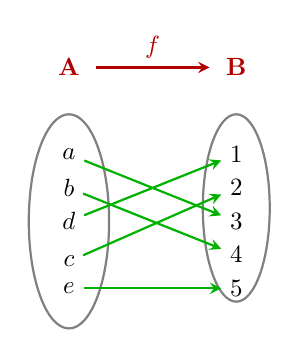
\begin{tikzpicture}[scale=0.85, every node/.style={scale=0.9}]

    % Ensembles A et B
    \node[text=darkred, font=\bfseries] at (0,2.3) {A};
    \node[text=darkred, font=\bfseries] at (2.5,2.3) {B};

    % Flèche de l'application
    \draw[->, >=stealth, color=darkred, thick]
        (0.4,2.3) -- node[above] {$f$} (2.1,2.3);

    % Patates A et B
    \draw[thick, color=gray]
        (0,0) ellipse (0.6cm and 1.6cm);

    \draw[thick, color=gray]
        (2.5,0.2) ellipse (0.5cm and 1.4cm);

    % Éléments de A
    \node (a) at (0,1.0) {$a$};
    \node (b) at (0,0.5) {$b$};
    \node (d) at (0,0.0) {$d$};
    \node (c) at (0,-0.6) {$c$};
    \node (e) at (0,-1.0) {$e$};

    % Éléments de B
    \node (b1) at (2.5,1.0) {$1$};
    \node (b2) at (2.5,0.5) {$2$};
    \node (b3) at (2.5,0.0) {$3$};
    \node (b4) at (2.5,-0.5) {$4$};
    \node (b5) at (2.5,-1.0) {$5$};

    % Flèches
    \draw[->, >=stealth, color=darkgreen, thick]
        (a) -- (b3);

    \draw[->, >=stealth, color=darkgreen, thick]
        (b) -- (b4);

    \draw[->, >=stealth, color=darkgreen, thick]
        (d) -- (b1);

    \draw[->, >=stealth, color=darkgreen, thick]
        (c) -- (b2);

    \draw[->, >=stealth, color=darkgreen, thick]
        (e) -- (b5);

\end{tikzpicture}

\end{center}

Chaque élément de $B$ a un et un seul antécédent par $f$ dans $A$.
Donc $f$ est une application bijective ou une bijection.


\bigskip


% =========================================================
% DIAGRAMME 2 : g : E \longrightarrow F
% =========================================================

\begin{center}

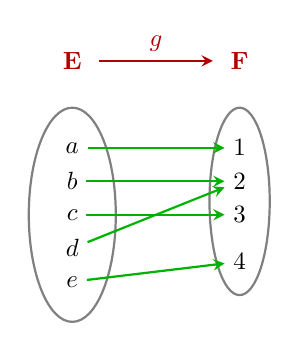
\begin{tikzpicture}[scale=0.85, every node/.style={scale=0.9}]

    % Ensembles E et F
    \node[text=darkred, font=\bfseries] at (0,2.3) {E};
    \node[text=darkred, font=\bfseries] at (2.5,2.3) {F};

    % Flèche de l'application
    \draw[->, >=stealth, color=darkred, thick]
        (0.4,2.3) -- node[above] {$g$} (2.1,2.3);

    % Patates E et F
    \draw[thick, color=gray]
        (0,0) ellipse (0.65cm and 1.6cm);

    \draw[thick, color=gray]
        (2.5,0.2) ellipse (0.45cm and 1.4cm);

    % Éléments de E
    \node (a) at (0,1.0) {$a$};
    \node (b) at (0,0.5) {$b$};
    \node (c) at (0,0.0) {$c$};
    \node (d) at (0,-0.5) {$d$};
    \node (e) at (0,-1.0) {$e$};

    % Éléments de F
    \node (f1) at (2.5,1.0) {$1$};
    \node (f2) at (2.5,0.5) {$2$};
    \node (f3) at (2.5,0.0) {$3$};
    \node (f4) at (2.5,-0.7) {$4$};

    % Flèches
    \draw[->, >=stealth, color=darkgreen, thick]
        (a) -- (f1);

    \draw[->, >=stealth, color=darkgreen, thick]
        (b) -- (f2);

    \draw[->, >=stealth, color=darkgreen, thick]
        (c) -- (f3);

    \draw[->, >=stealth, color=darkgreen, thick]
        (d) -- (f2);

    \draw[->, >=stealth, color=darkgreen, thick]
        (e) -- (f4);

\end{tikzpicture}

\end{center}

$2$ admet deux antécédents donc $g$ n'est pas une application bijective.


\bigskip


% =========================================================
% DIAGRAMME 3 : h : M \longrightarrow N
% =========================================================

\begin{center}

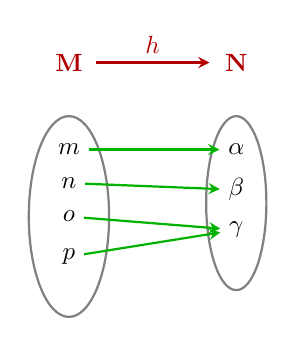
\begin{tikzpicture}[scale=0.85, every node/.style={scale=0.9}]

    % Ensembles M et N
    \node[text=darkred, font=\bfseries] at (0,2.3) {M};
    \node[text=darkred, font=\bfseries] at (2.5,2.3) {N};

    % Flèche de l'application
    \draw[->, >=stealth, color=darkred, thick]
        (0.4,2.3) -- node[above] {$h$} (2.1,2.3);

    % Patates M et N
    \draw[thick, color=gray]
        (0,0) ellipse (0.6cm and 1.5cm);

    \draw[thick, color=gray]
        (2.5,0.2) ellipse (0.45cm and 1.3cm);

    % Éléments de M
    \node (m) at (0,1.0) {$m$};
    \node (n) at (0,0.5) {$n$};
    \node (o) at (0,0.0) {$o$};
    \node (p) at (0,-0.6) {$p$};

    % Éléments de N
    \node (alpha) at (2.5,1.0) {$\alpha$};
    \node (beta) at (2.5,0.4) {$\beta$};
    \node (gamma) at (2.5,-0.2) {$\gamma$};

    % Flèches
    \draw[->, >=stealth, color=darkgreen, thick]
        (m) -- (alpha);

    \draw[->, >=stealth, color=darkgreen, thick]
        (n) -- (beta);

    \draw[->, >=stealth, color=darkgreen, thick]
        (o) -- (gamma);

    \draw[->, >=stealth, color=darkgreen, thick]
        (p) -- (gamma);

\end{tikzpicture}

\end{center}

$\gamma$ n'a pas d'antécédent par $h$.

Donc, $h$ n'est pas une bijection.

\subsubsection*{\underline{\textbf{Applications}}}

\begin{enumerate}

    \item Soit $f$ l'application  définie par
    
\[
\begin{array}{rcl}
f:[0\,;\,+\infty[ & \longrightarrow & [0\,;\,+\infty[\\
x                 & \longmapsto      & f(x)=x^2
\end{array}
\]

    $f$ est-elle bijective ?

    Soit $y\in[0\,;\,+\infty[$, résolvons l'équation $f(x)=y$.

    \[
    f(x)=y
    \Longrightarrow x^2=y
    \Longrightarrow x=\sqrt{y}\in[0\,;\,+\infty[\quad \text{ou}\quad x=-\sqrt{y}\notin[0\,;\,+\infty[
    \]

    Donc l'équation $f(x)=y$ admet une unique solution $x=\sqrt{y}.$

    Par conséquent, $f$ est une \textcolor{darkred}{bijection}.


    \item Soit $\ell$ la relation définie par :
    \[
	\begin{array}{rcl}
	\ell:]-\infty\,;\,-2] & \longrightarrow & [-3\,;\,+\infty[\\
		x                 & \longmapsto      & \ell(x)=x^2+4x+1
	\end{array}
	\]

    \begin{enumerate}
        \item $\ell$ est-elle une application ?

        \item Si oui, est-elle bijective ?
    \end{enumerate}


    \begin{enumerate}

        \item Soit $x\in]-\infty\,;\,-2]$, il est clair que
        $x^2+4x+1$ est unique car $ x^2+4x+1=(x+2)^2-3. $

        De plus,
        $
            (x+2)^2\geq 0
            \Longrightarrow
            (x+2)^2-3\geq -3.
        $

        Ce qui donne
        $
            \ell(x)\geq -3
            \Longrightarrow
            \ell(x)\in[-3\,;\,+\infty[.
        $

        Par conséquent, $\ell$ est une \textcolor{darkred}{application}.


        \bigskip

        \begin{center}
            \underline{\textbf{\textcolor{darkred}{OU}}}
        \end{center}

        Soit $x\in]-\infty\,;\,-2]$, il est clair que
        $x^2+4x+1$ est unique.

        Vérifions que si $\ell(x)\geq -3$.

        Pour cela, évaluons $\ell(x)+3$.

        $
          \begin{aligned}
          \ell(x)+3&=x^2+4x+1+3\\
          		&=x^2+4x+4
          \end{aligned}
        $

        $
            \ell(x)+3=(x+2)^2\geq 0
        $

        $
            \ell(x)+3\geq 0
            \Longrightarrow
            \ell(x)\geq -3
       $

        Donc,
        $
            	\ell(x)\in[-3\,;\,+\infty[.
        $

        Par conséquent, $\ell$ est une \textcolor{darkred}{application}.


        \item Soit $y\in[-3\,;\,+\infty[$, résolvons $\ell(x)=y$.
        
        $
		\begin{aligned}
		x^2+4x+1=y &\Longrightarrow x^2+4x+1-y=0\\
		                     &\Delta=16-4(1)(1-y)\\
		                     &\Delta=16-4+4y\\
		                     &\Delta=12+4y		                     
		\end{aligned}        
        $

$
\text{Posons} \Delta=0
$\\

$
12+4y=0
\quad\Longrightarrow\quad
y=-3
$

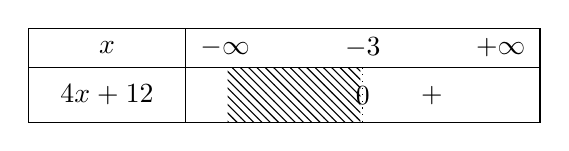
\begin{tikzpicture}[node style/.style={fill opacity=0,text opacity=1}]
    \tkzTabInit[
        espcl=1.75
    ]{$x$/.5,$4x+12$/.7}
    {$-\infty$,$-3$,$+\infty$}
    \tkzTabLine{,h,z,+,}
\end{tikzpicture}

$
\text{car } y\in[-3\,;\,+\infty[
$

Comme $\Delta>0$, l'équation $\ell(x)=y$ admet 2 solutions.

\bigskip

\underline{\textbf{Si $y=3$}} alors $\Delta=0$ ;
$
x_0=\dfrac{-4}{2}=-2.
$

\bigskip

\underline{\textbf{Si $y>-3$}}

$
x_1=
\dfrac{-4-\sqrt{12+4y}}{2}
=
\dfrac{-4-\sqrt{4(3+y)}}{2}
=
-2-\sqrt{3+y}
<-2
$

$
x_2=-2+\sqrt{3+y}>-2
\qquad \text{alors}
$

$
x_2\notin]-\infty\,;\,-2].
$

\[
\boxed{x_1=-2-\sqrt{3+y}\in]-\infty\,;\,-2]}
\]

\bigskip

\underline{\textbf{Conclusion :}}

$
\forall y\in]-3\,;\,+\infty[,
\quad
\text{l'équation }\ell(x)=y
\text{ admet une unique solution}
$
$
\text{dans }]-\infty\,;\,-2].
$

Donc, $\ell$ est une \textcolor{darkred}{application bijective}.
    \end{enumerate}

\end{enumerate}

\subsubsection*{\textbf{c) Bijections réciproques :}}

\paragraph{\color{darkred} Définition :}~\\

$f$ étant une bijection d'un ensemble $A$ dans un ensemble $B$, on appelle
\textcolor{darkred}{\textbf{bijection réciproque de $f$}}, l'application
de $B$ dans $A$ notée $f^{-1}$ qui à tout élément de $B$ associe son
unique antécédent par $f$ dans $A$.

L'application réciproque est définie de l'ensemble d'arrivée $B$ vers
l'ensemble de départ $A$.

\paragraph{\color{darkred} Propriété :}~\\

Si $f^{-1}$ est l'application de $f$, alors $f$ est aussi l'application
réciproque de $f^{-1}$.

\paragraph{\color{darkred} Ex :}~\\

On donne :
\[
\begin{array}{rcl}
f:\mathbb{R}\setminus\{-3\} & \longrightarrow &
\mathbb{R}\setminus\{2\}\\
x & \longmapsto &
\dfrac{2x+1}{x+3}
\end{array}
\]

Montrer que $f$ est une bijection puis déterminer sa bijection
réciproque.

\paragraph{\color{darkred} Résolution :}~\\

Montrons que $f$ est une bijection puis déterminons sa bijection
réciproque.

Soit $y\in\mathbb{R}\setminus\{2\}$, résolvons $f(x)=y$.

\[
\begin{aligned}
f(x)=y &\Longrightarrow \frac{2x+1}{x+3}=y\\
       &\Longrightarrow 2x+1=yx+3y \\
       &\Longrightarrow 2x-xy=3y-1\\
       &\Longrightarrow x(2-y)=3y-1\\
       &\Longrightarrow x=\frac{3y-1}{2-y}
\end{aligned}
\]

Comme $y\neq2$ donc $x=\frac{3y-1}{2-y}$ existe et est unique.

Montrons que $ x\in\mathbb{R}\setminus\{-3\}, $
pour cela on pose

\[
\begin{aligned}
\frac{3y-1}{2-y}=-3 &\Longrightarrow 3y-1=-6+3y\\
       &\Longrightarrow -1=-6 \\
       &\Longrightarrow \text{absurde !!}
\end{aligned}
\]

Par conséquent,$ \frac{3y-1}{2-y}\neq-3 $

Ce qui donne l'équation $f(x)=y$ admet une unique solution
\[
x=\frac{3y-1}{2-y}\in\mathbb{R}\setminus\{-3\}.
\]

D'où $f$ est une \textcolor{darkred}{bijection} et admet donc
une bijection réciproque notée :

\[ 
\begin{array}{rcl}
f^{-1}:\mathbb{R}\setminus\{2\} & \longrightarrow & \mathbb{R}\setminus\{-3\}\\
y & \longmapsto & f^{-1}(y)=\frac{3y-1}{2-y}
\end{array}
\]


Comme la variable est muette, $\boxed{
f^{-1}(x)=\frac{3x-1}{2-x}
}$

\subsection*{\underline{\textbf{\textcolor{darkgreen}{3) Application injective ou injection}}}}

\subsubsection*{\underline{\textbf{a) Définition :}}}

Une application $f$ définie de $A$ vers $B$ est dite
\textcolor{darkred}{\textbf{injective}} (on dit que $f$ est une injection)
si chaque élément de $B$ est l'image au plus par $f$ d'un élément de $A$.

C'est-à-dire pour tout $y\in B$, l'équation $f(x)=y$ admet au plus une solution.


\subsubsection*{\textbf{b) Propriété :}}

\begin{itemize}
    \item Pour montrer qu'une application $f$ définie de $A$ vers $B$ est injective,
    il suffit de montrer que pour tout $x\in A$ et $x'\in A$ tel que $ f(x)=f(x'),$
    on ait $x=x'.$

    \item Pour montrer qu'une application $f$ définie de $A$ vers $B$ n'est pas injective,
    il suffit de trouver deux éléments $x$ et $x'$ dans $A$ tels que $ x\neq x'
        \qquad\text{et}\qquad
        f(x)=f(x').$
\end{itemize}

\subsubsection*{\underline{\textbf{\textcolor{darkred}{Illustration graphique}}}}

\begin{center}

% --- DIAGRAMME 1 : h ---

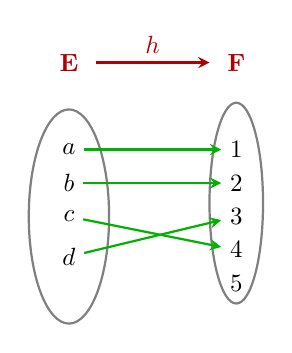
\begin{tikzpicture}[scale=0.85, every node/.style={scale=0.9}]

    % Ensembles E et F
    \node[text=darkred, font=\bfseries] at (0,2.3) {E};
    \node[text=darkred, font=\bfseries] at (2.5,2.3) {F};

    % Flèche indiquant l'application
    \draw[->, >=stealth, color=darkred, thick]
        (0.4,2.3) -- node[above] {$h$} (2.1,2.3);

    % Patates E et F
    \draw[thick, color=gray]
        (0,0) ellipse (0.6cm and 1.6cm);

    \draw[thick, color=gray]
        (2.5,0.2) ellipse (0.4cm and 1.5cm);

    % Éléments de E
    \node (a) at (0,1.0) {$a$};
    \node (b) at (0,0.5) {$b$};
    \node (c) at (0,0.0) {$c$};
    \node (d) at (0,-0.6) {$d$};

    % Éléments de F
    \node (f1) at (2.5,1.0) {$1$};
    \node (f2) at (2.5,0.5) {$2$};
    \node (f3) at (2.5,0.0) {$3$};
    \node (f4) at (2.5,-0.5) {$4$};
    \node (f5) at (2.5,-1.0) {$5$};

    % Flèches
    \draw[->, >=stealth, color=darkgreen, thick]
        (a) -- (f1);

    \draw[->, >=stealth, color=darkgreen, thick]
        (b) -- (f2);

    \draw[->, >=stealth, color=darkgreen, thick]
        (c) -- (f4);

    \draw[->, >=stealth, color=darkgreen, thick]
        (d) -- (f3);

\end{tikzpicture}

\end{center}

On constate que chaque élément de $F$ est l'image au plus d'un élément de $E$.
Par suite, $h$ est une injection.


\bigskip

\begin{center}

% --- DIAGRAMME 2 : f ---

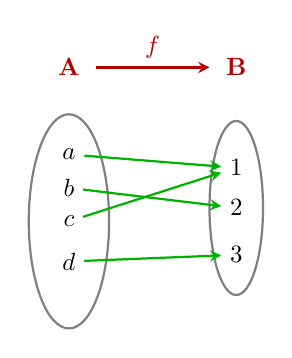
\begin{tikzpicture}[scale=0.85, every node/.style={scale=0.9}]

    % Ensembles A et B
    \node[text=darkred, font=\bfseries] at (0,2.3) {A};
    \node[text=darkred, font=\bfseries] at (2.5,2.3) {B};

    % Flèche indiquant l'application
    \draw[->, >=stealth, color=darkred, thick]
        (0.4,2.3) -- node[above] {$f$} (2.1,2.3);

    % Patates A et B
    \draw[thick, color=gray]
        (0,0) ellipse (0.6cm and 1.6cm);

    \draw[thick, color=gray]
        (2.5,0.2) ellipse (0.4cm and 1.3cm);

    % Éléments de A
    \node (a) at (0,1.0) {$a$};
    \node (b) at (0,0.5) {$b$};
    \node (c) at (0,0.0) {$c$};
    \node (d) at (0,-0.6) {$d$};

    % Éléments de B
    \node (b1) at (2.5,0.8) {$1$};
    \node (b2) at (2.5,0.2) {$2$};
    \node (b3) at (2.5,-0.5) {$3$};

    % Flèches
    \draw[->, >=stealth, color=darkgreen, thick]
        (a) -- (b1);

    \draw[->, >=stealth, color=darkgreen, thick]
        (b) -- (b2);

    \draw[->, >=stealth, color=darkgreen, thick]
        (c) -- (b1);

    \draw[->, >=stealth, color=darkgreen, thick]
        (d) -- (b3);

\end{tikzpicture}

\end{center}

Comme $f(a)=f(c)=1$, donc $f$ n'est pas une injection.

\subsubsection*{\underline{\textbf{Applications :}}}

\textbf{A1 :}
Soit\\
\(
\begin{array}{rcl}
f:\mathbb{R}\setminus\{-3\} & \longrightarrow &
\mathbb{R}\setminus\{2\}\\
x & \longmapsto &
\dfrac{2x+1}{x+3}
\end{array}
\)

Montrer que $f$ est une injection.


\bigskip

\textbf{A2 :}

Soit 

\(
\begin{array}{rcl}
f:\mathbb{R} & \longrightarrow & \mathbb{R}\\
x & \longmapsto & x^2-4x+3
\end{array}
\)

$f$ est-elle une injection ?


\subsubsection*{\textcolor{darkred}{Résolution :}}

\textbf{A1 :}

Montrons que $f$ est une injection.

Soit $x\in\mathbb{R}\setminus\{-3\}$ et
$x'\in\mathbb{R}\setminus\{-3\}$.

Résolvons $f(x)=f(x')$.

\[
\begin{aligned}
f(x)=f(x')
&\Longleftrightarrow
\frac{2x+1}{x+3}
=
\frac{2x'+1}{x'+3}\\
&\Longrightarrow
(2x+1)(x'+3)
=
(2x'+1)(x+3)\\
&\Longrightarrow
2xx'+6x+x'+3
=
2xx'+6x'+x+3\\
&\Longrightarrow
5x'=5x\\
&\Longrightarrow
x'=x
\end{aligned}
\]

Par conséquent $f$ est une injection.
\end{document}
